
\definecolor{ublue}{rgb}{0.152,0.250,0.545}
\definecolor{ugreen}{rgb}{0,0.5,0}


%%% outline
%-------------------------------------------------------------------------

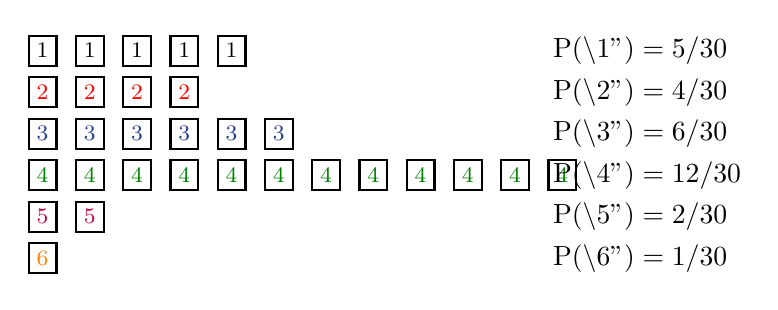
\begin{tikzpicture}[scale=0.6]
\begin{scope}
{\footnotesize
\foreach \i in {1,...,5}{
    \node [draw,thick,minimum size=10pt] at (\i,0) {1};
}
}
\node [anchor=west] at (33em,0) {$\textrm{P}(\text{“1”}) = 5/30$};
\end{scope}

\begin{scope}[yshift=-2.5em]
{\footnotesize
\foreach \i in {1,...,4}{
    \node [draw,thick,minimum size=10pt] at (\i,0) {{\color{red} 2}};
}
}
\node [anchor=west] at (33em,0) {$\textrm{P}(\text{“2”}) = 4/30$};
\end{scope}

\begin{scope}[yshift=-5.0em]
{\footnotesize
\foreach \i in {1,...,6}{
    \node [draw,thick,minimum size=10pt] at (\i,0) {{\color{ublue} 3}};
}
}
\node [anchor=west] at (33em,0) {$\textrm{P}(\text{“3”}) = 6/30$};
\end{scope}

\begin{scope}[yshift=-7.5em]
{\footnotesize
\foreach \i in {1,...,12}{
    \node [draw,thick,minimum size=10pt] at (\i,0) {{\color{ugreen} 4}};
}
}
\node [anchor=west] at (33em,0) {$\textrm{P}(\text{“4”}) = 12/30$};
\end{scope}

\begin{scope}[yshift=-10.0em]
{\footnotesize
\foreach \i in {1,...,2}{
    \node [draw,thick,minimum size=10pt] at (\i,0) {{\color{purple} 5}};
}
}
\node [anchor=west] at (33em,0) {$\textrm{P}(\text{“5”}) = 2/30$};
\end{scope}

\begin{scope}[yshift=-12.5em]
{\footnotesize
\foreach \i in {1,...,1}{
    \node [draw,thick,minimum size=10pt] at (\i,0) {{\color{orange} 6}};
}
}
\node [anchor=west] at (33em,0) {$\textrm{P}(\text{“6”}) = 1/30$};
\end{scope}

\end{tikzpicture}




